%%%%%%%%%%%%%%%%%%%%%%%%%%%%%%%%%%%%%%%%%
% University/School Laboratory Report
% LaTeX Template
% Version 3.1 (25/3/14)
%
% This template has been downloaded from:
% http://www.LaTeXTemplates.com
%
% Original author:
% Linux and Unix Users Group at Virginia Tech Wiki 
% (https://vtluug.org/wiki/Example_LaTeX_chem_lab_report)
%
% License:
% CC BY-NC-SA 3.0 (http://creativecommons.org/licenses/by-nc-sa/3.0/)
%
%%%%%%%%%%%%%%%%%%%%%%%%%%%%%%%%%%%%%%%%%

%----------------------------------------------------------------------------------------
%	PACKAGES AND DOCUMENT CONFIGURATIONS
%----------------------------------------------------------------------------------------

\documentclass{article}

\usepackage[version=3]{mhchem} % Package for chemical equation typesetting
\usepackage{siunitx} % Provides the \SI{}{} and \si{} command for typesetting SI units
\usepackage{graphicx} % Required for the inclusion of images
\usepackage{natbib} % Required to change bibliography style to APA
\usepackage{amsmath} % Required for some math elements 
\usepackage[utf8]{inputenc}
\usepackage[margin=1.2in]{geometry}

\setlength\parindent{0pt} % Removes all indentation from paragraphs

% \renewcommand{\labelenumi}{\alph{enumi}.} % Make numbering in the enumerate environment by letter rather than number (e.g. section 6)

\renewcommand{\figurename}{Figura}
\renewcommand{\tablename}{Tabla}
\renewcommand\refname{Referencias}

\def\mean#1{\left< #1 \right>}
%\usepackage{times} % Uncomment to use the Times New Roman font

%----------------------------------------------------------------------------------------
%	DOCUMENT INFORMATION
%----------------------------------------------------------------------------------------

\title{M\'etodos num\'ericos para la Ciencia e Ingenier\'ia \\ Tarea 6: Métodos Aleatorios} % Title

\author{Felipe Toledo Bittner} % Author name

\date{\today} % Date for the report

\begin{document}

\maketitle % Insert the title, author and date

%----------------------------------------------------------------------------------------
%	SECTION 1
%----------------------------------------------------------------------------------------

\section{Integración de Montecarlo}

\subsection{Introducción}
\label{sec:introduccion_P1}

Se desea obtener la posición del centro de masa de un sólido formado por la intersección de un toro con un cilindro, descrito por las ecuaciones (\ref{eq:toro}) y (\ref{eq:cilindro}).

\begin{equation}
  Toro:\ z^2 + \left( \sqrt{x^2 + y^2} - 3 \right)^2 \leq 1
  \label{eq:toro}
\end{equation}

\begin{equation}
  Cilindro:\ (x - 2)^2 + z^2 \leq 1
  \label{eq:cilindro}
\end{equation}

La densidad del sólido no es uniforme y es descrita por la fórmula (\ref{eq:densidad}). Debido a esto último, realizar una integración analítica para encontrar el centro de masa puede resultar complejo, por lo que se decide utilizar el método numérico de Monte Carlo para estimar su posición.

\begin{equation}
  \rho(x, y, z) = 0.5 (x^2 + y^2 + z^2)
  \label{eq:densidad}
\end{equation}

Las integrales que se deben calcular para obtener la coordenada $x^i$ del centro de masa son las siguientes:

\begin{equation}
  M = \int_V \rho(\vec{r}) dx dy dz \approx \sum_j \rho(\vec{r_j}) \Delta V
  \label{eq:calculo_masa}
\end{equation}

\begin{equation}
  T^i = \int_V x^i \rho(\vec{r}) dx dy dz \approx \sum_j x_j \rho(\vec{r_j}) \Delta V
  \label{eq:calculo_torque}
\end{equation}


En este caso $V$ es el volumen del cuerpo, condición que será relajada para el cálculo numérico y $\Delta V \approx \frac{V}{N}$, con $N$ la cantidad de términos en la suma. El cálculo de $x_i$ se realiza de la forma indicada en la ecuación (\ref{eq:error}). Como cada integral obtenida con el método de Monte Carlo posee un error asociado, este se propagará quedando $x^i = \mean{x^i} \pm \Delta x^i$.

\begin{equation}
  x^i = \frac{\mean{T^i} + \Delta T^i}{\mean{M} + \Delta M} = \frac{\mean{T^i}}{\mean{M}} \pm \frac{\mean{T^i}}{\mean{M}} \sqrt{ \left( \frac{\Delta T^i}{\mean{T^i}} \right)^2 + \left( \frac{\Delta M}{\mean{M}} \right)^2 }
  \label{eq:error}
\end{equation}

\subsection{Implementación}

Para usar el algoritmo de Monte Carlo, resulta útil definirse un volumen $W$ que contenga a $V$, pero posea una geometría mas sencilla. Para este caso se utilizará un $W$ con forma de caja rectangular que acote de forma lo más precisa posible al sólido en estudio.

En la Figura \ref{fig:interseccion_P1} se puede ver que el volumen del sólido está contenido en $ [-1 \le z \le 1]$ y $[1 \le x \le 3]$. Realizando un despeje sencillo en $x = 1$, $z = 0$ se pueden obtener los valores extremos de $y$, que son $y^* = \pm \sqrt{15}$. Como se realizan integrales sobre volumen, el error por la resolución de los números de punto flotante debiese resultar despreciable, por lo que se decide usar el intervalo $[-\sqrt{15} \le y \le \sqrt{15} ]$ para terminar de definir el volumen $W$.

\begin{figure}[ht]
  \centering
  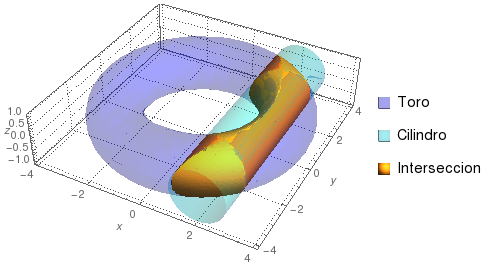
\includegraphics[scale = 0.5]{images/interseccion_P1.png}
  \caption{La figura naranja es el sólido en estudio. Está formado por el volumen que se obtiene al intersectar el toro (celeste) con el cilindro (azul) descritos en la Sección \ref{sec:introduccion_P1}. La rutina del programa \emph{Mathematica} usada para hacer este dibujo se encuentra adjunta al repositorio.}
  \label{fig:interseccion_P1}
\end{figure}

En este volumen $W$ se usa el método de Monte Carlo, evaluando puntos generados al azar mediante una distribución uniforme, acotada por los intervalos correspondientes a cada coordenada. En caso de que un punto caiga fuera del sólido, se define $\rho = 0$ para anular su contribución a la integral.

\subsection{Resultados}

Realizando el cálculo con $N = 10^6$ se obtienen los valores de la Tabla \ref{tab:resultados}. Al comparar con la Figura \ref{fig:interseccion_P1} se observa que las coordenadas calculadas para el centro de masa están en el espacio ocupado por el sólido y parecen razonables.

\begin{table}[hl]
\centering
\begin{tabular}{|c|c|c|}
\hline
  Parámetro & Resultado \\
  \hline
  $M$ & $71.00 \pm 0.08$  \\ \hline
  $x_{CM}$ & $2.081 \pm 0.003$\\ \hline
  $y_{CM}$ & $0.001 \pm 0.003$\\ \hline
  $z_{CM}$ & $1 \cdot 10^{-4} \pm 7 \cdot 10^{-4}$\\ \hline
\end{tabular}
\caption{Tabla con resultados del cálculo numérico para la masa $M$ y las coordenadas del centro de masa $x^i_{CM}$.}
\label{tab:resultados}
\end{table}

\subsection{Conclusiones}

En esta ocasión la principal ventaja del método de Monte Carlo ha sido su fácil implementación. Bastó conocer las ecuaciones que acotaban el volumen de integración para poder realizar integración de funciones dentro de él, en este caso de densidad.

Como el algoritmo usado requiere una elevada cantidad de muestras para entregar resultados fiables (en este caso se usaron $10^6$ muestras), hay que tener especial cuidado en acotar lo máximo posible el volumen de pruebas o usar técnicas de optimización para limitar el tiempo de cómputo, que parece ser su principal limitante.

\section{Algoritmo de Metrópolis}

\subsection{Introducción}

Se desea obtener una muestra aleatoria de números que posean la distribución de la ecuación (\ref{eq:distribucion_no_normalizada}). Se desconoce la constante de normalizaciónde la distribución por lo que se utiliza el algoritmo de metrópolis para obtener los datos.

\begin{equation}
  W(x) = 3.5 \times \exp\left({\frac{-(x-3)^2}{3}}\right) + 2 \times \exp{\left(\frac{-(x+1.5)^2}{0.5}\right)}
  \label{eq:distribucion_no_normalizada}
\end{equation}

\subsection{Implementación}

Como el algoritmo de metrópolis requiere, para iniciar, de los parámetros posición inicial y tamaño máximo de paso, primero se grafica la distribución no normalizada para observar su forma, obteniéndose la Figura \ref{fig:distribucion_no_norm}.

\begin{figure}[ht]
  \centering
  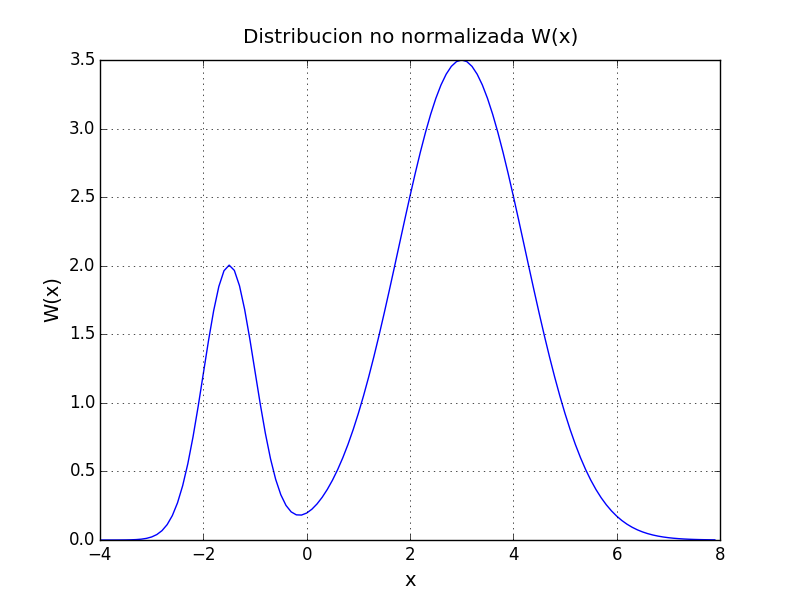
\includegraphics[scale = 0.5]{images/distribucion_no_normalizada.png}
  \caption{Gráfico de la función $W(x)$. Fuera de la imagen la función continúa su decaimiento exponencial.}
  \label{fig:distribucion_no_norm}
\end{figure}

Se puede ver de la imagen que existe la posibilidad de que el paso tenga problemas en atravesar de un lado a otro de la función en torno a $ x = 0 $, por lo que se usa un paso máximo $d = 2$. Como posición inicial se escoge $x_0 = 0$.

Para comparar estos resultados con la distribución original, se normaliza $W(x)$ dividiéndola por su área calculada integrando numéricamente con el método de los trapecios en el intervalo $x \in [-70, 100]$.

\clearpage
\subsection{Resultados}

Usando los valores escogidos en la sección anterior, se obtiene la distribución de muestras de la Figura \ref{fig:resultados}, con una tasa de acierto de $\approx 66\%$.

\begin{figure}[ht]
  \centering
  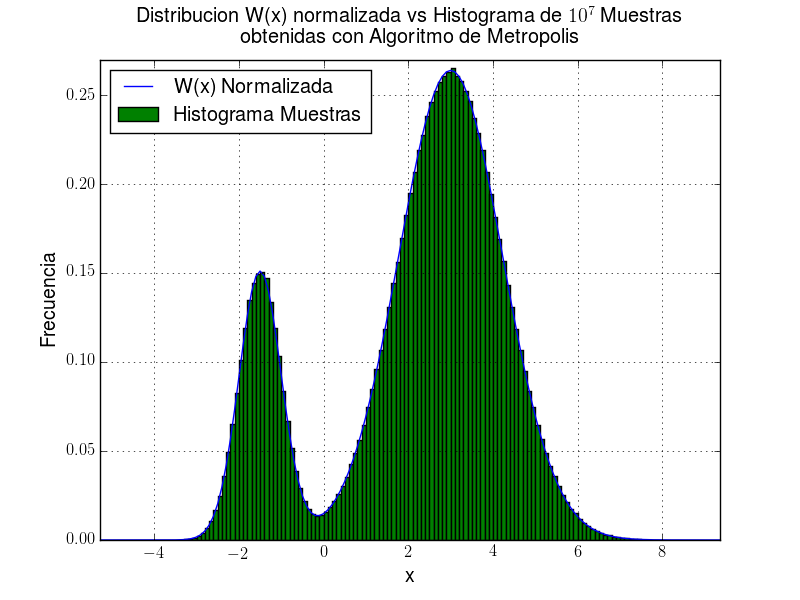
\includegraphics[scale = 0.65]{images/resultado_P2.png}
  \caption{Gráfico de la función $W(x)$ normalizada vs un histograma con las muestras obtenidas del Algoritmo de Metrópolis. Las barras son de ancho $dx = 0.1$ y están definidas en el intervalo $x \in [-6, 10]$.}
  \label{fig:resultados}
\end{figure}

La imagen permite inferir que efectivamente se logró generar números aleatorios con una distribución equivalente a la de $W(x)$, al menos para los puntos donde esta última alcanza sus valores más elevados.

\subsection{Error}

Para determinar el error de cada bin del histograma, se procede realizando muchas iteraciones del algoritmo con parámetros iniciales distintos. Los parámetros se varían usando distribuciones aleatorias uniformes $U(x_{min}, x_{max}$), de la siguiente manera:

\begin{itemize}
  \item Posicion inicial $ x_0 = U(-1 , 1) $ 
  
  \item Distancia máxima de paso $ d = U(0.5, 3) $
\end{itemize}

Los valores se escogieron de forma que resulten similares a los utilizados en la iteración original (que dieron buenos resultados), pero con variación suficiente para revisar si el primer criterio utilizado fue muy arbitrario. La Figura \ref{fig:bonus} muestra los resultados obtenidos. El error usado es la desviación estándar del valor de cada barra considerando todas las muestras calculadas.

\begin{figure}[ht]
  \centering
  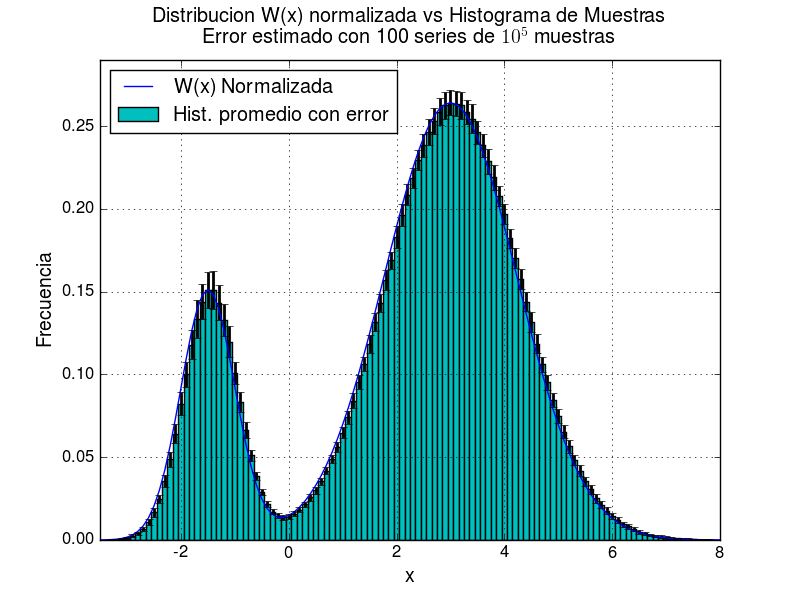
\includegraphics[scale = 0.65]{images/bonus_P2.png}
  \caption{Histograma con barras de error. Se observa que la variación es mayor en los puntos más probables, lo que tiene sentido ya que son obtenidos con más frecuencia respecto a los menos probables. El error puede disminuirse aumentando el número de muestras por iteración.}
  \label{fig:bonus}
\end{figure}

La cantidad de muestras por iteración fue disminuida debido al tiempo de cálculo requerido, sin embargo el histograma se grafica usando el promedio de todos los resultados por lo que existe cierta compensación. 


\subsection{Conclusiones}

El algoritmo implementado demostró ser exigente computacionalmente durante las simulaciones. Posiblemente se debe a que requiere un repetido cálculo de valores estocásticos, lo que sumado a la gran cantidad de iteraciones necesarias repercuten en un tiempo de procesamiento elevado. Considerando que el Algoritmo de Metrópolis es una cadena de Markov Monte Carlo, la última característica indica que al parecer los algoritmos de esta familia son exigentes, aunque se debe realizar más investigación para verificarlo. 

También resulta importante notar que, pese a que $W(x) > 0$ en todos los puntos, no se obtuvieron muestras de $x$ muy lejanas a los puntos elevados de la distribución. El motivo es que el tamaño de paso acotado junto a la condición de aprobación de punto acotan la máxima distancia que el algoritmo puede avanzar en las zonas de baja probabilidad, por lo que esta técnica aproxima mejor a $W(x)$ para los valores de mayor probabilidad. Aun más, existen valores muy improbables pero posibles que se pueden obtener de $W(x)$ que podrían estar sub-representados o no aparecer en la estimación numérica.

Del gráfico del error (Figura \ref{fig:bonus} se puede concluir que el método posee una incertidumbre no uniforme en el cálculo, con acentuación en los valores más probables. Esto quiere decir que es más probable sobreestimar o subestimar la frecuencia de aparición de estos valores mediante el método de Metrópolis. De todas formas la incertidumbre puede disminuirse aumentando la cantidad de muestras, con el costo de mayor tiempo de cálculo por supuesto.

\end{document}
